% --------------------------------------------------------------
% This is all preamble stuff that you don't have to worry about.
% Head down to where it says "Start here"
% --------------------------------------------------------------
 
\documentclass[12pt]{article}
 
\usepackage{listings}
\usepackage{hyperref}
\usepackage{color}
\definecolor{lightgray}{rgb}{.95,.95,.95}
\definecolor{darkgray}{rgb}{.4,.4,.4}
\definecolor{purple}{rgb}{0.65, 0.12, 0.82}

\lstdefinelanguage{JavaScript}{
  keywords={typeof, new, true, false, catch, function, return, null, catch, switch, var, if, in, while, do, else, case, break},
  keywordstyle=\color{blue}\bfseries,
  ndkeywords={class, export, boolean, throw, implements, import, this},
  ndkeywordstyle=\color{darkgray}\bfseries,
  identifierstyle=\color{black},
  sensitive=false,
  comment=[l]{//},
  morecomment=[s]{/*}{*/},
  commentstyle=\color{purple}\ttfamily,
  stringstyle=\color{red}\ttfamily,
  morestring=[b]',
  morestring=[b]"
}

\lstset{
   language=JavaScript,
   backgroundcolor=\color{lightgray},
   extendedchars=true,
   basicstyle=\footnotesize\ttfamily,
   showstringspaces=false,
   showspaces=false,
   numbers=left,
   numberstyle=\footnotesize,
   numbersep=9pt,
   tabsize=2,
   breaklines=true,
   showtabs=false,
   captionpos=b
}

\usepackage[margin=1in]{geometry} 
\usepackage{amsmath,amsthm,amssymb}
\usepackage{graphicx}%
\usepackage{float}
\newcommand{\N}{\mathbb{N}}
\newcommand{\Z}{\mathbb{Z}}
 
% --------------------------------------------------------------
%                         Start here
% --------------------------------------------------------------
 
\title{Documentation Pet Project}%replace X with the appropriate number
\author{Christoph Geis-Schroer\\ %replace with your name
Advanced Softwareengineering} %if necessary, replace with your course title
 \begin{document}
\maketitle

\section{Introduction}

The idea for the pet project \url{https://github.com/chrisschroer/pet_project} was to develop a prototype for an app which guides through the nighlife of a city, e.g. Berlin. In the following pictures, screenshots of the prototype are shown, e.g. the Home page with the club and event overview or the Blood Alochol page, where a user could roughly calculate his/her blood alcohol level based on the drinking behaviour.

\begin{figure}[H]
\minipage{0.32\textwidth}
  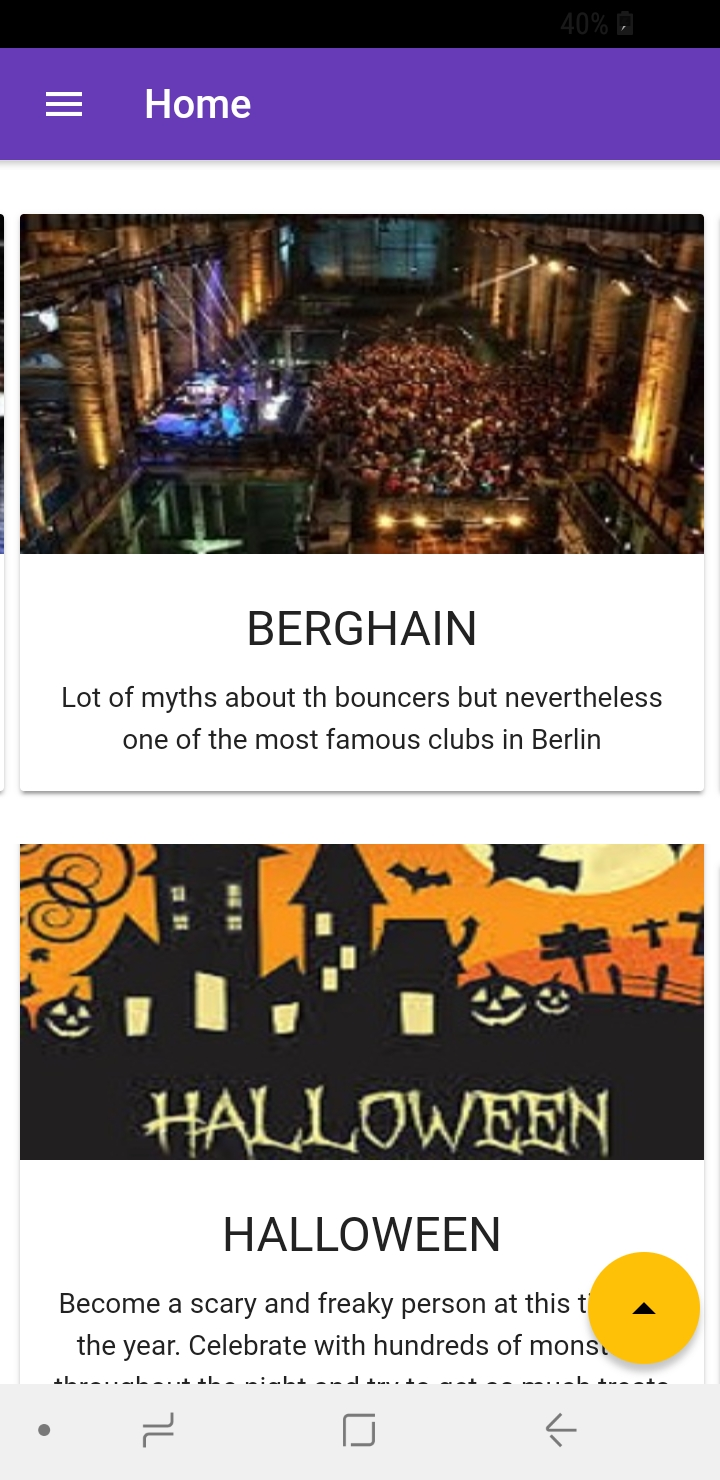
\includegraphics[width=\linewidth]{figures/Main.jpg}
  \caption{Starting Page}\label{fig:awesome_image1}
\endminipage\hfill
\minipage{0.32\textwidth}
  
\includegraphics[width=\linewidth]{figures/Favorites.jpg}
  \caption{Favorites Page}\label{fig:awesome_image2}
\endminipage\hfill
\minipage{0.32\textwidth}%
  
\includegraphics[width=\linewidth]{figures/Favorites_delete.jpg}
  \caption{Delete Favorites}\label{fig:awesome_image3}
\endminipage
\end{figure}

\begin{figure}[H]
\minipage{0.32\textwidth}
  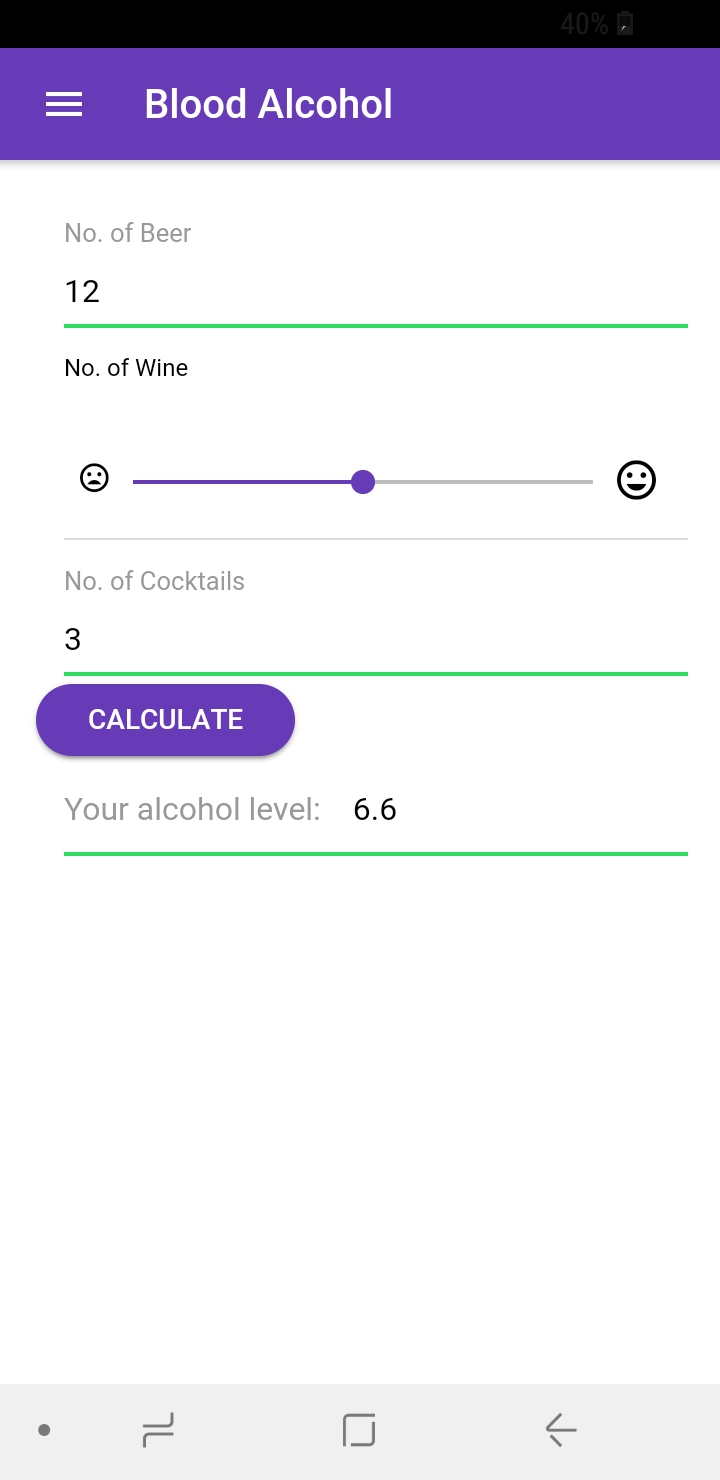
\includegraphics[width=\linewidth]{figures/Calc_alc.jpg}
  \caption{Blood alcohol page}\label{fig:awesome_image4}
\endminipage\hfill
\minipage{0.32\textwidth}
  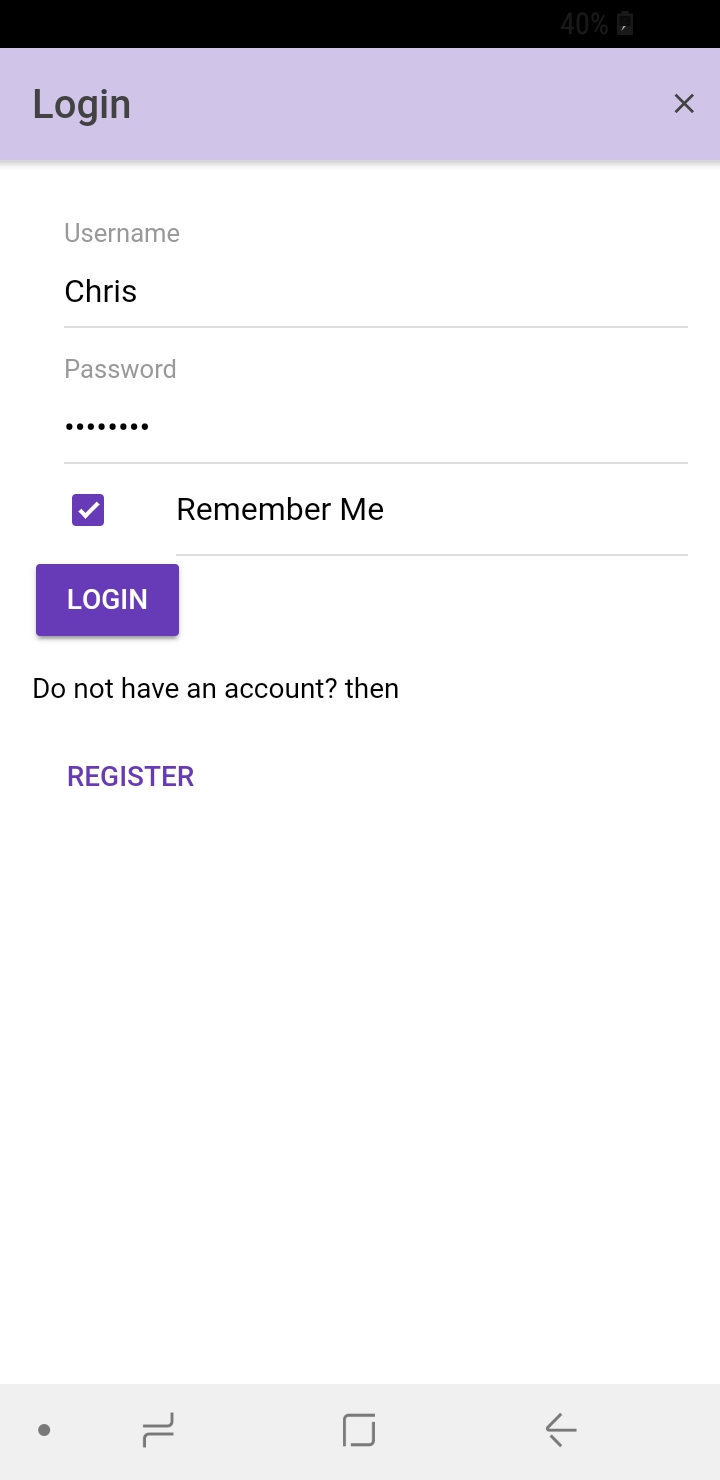
\includegraphics[width=\linewidth]{figures/Login.jpg}
  \caption{Login Page}\label{fig:awesome_image5}
\endminipage\hfill
\minipage{0.32\textwidth}%
  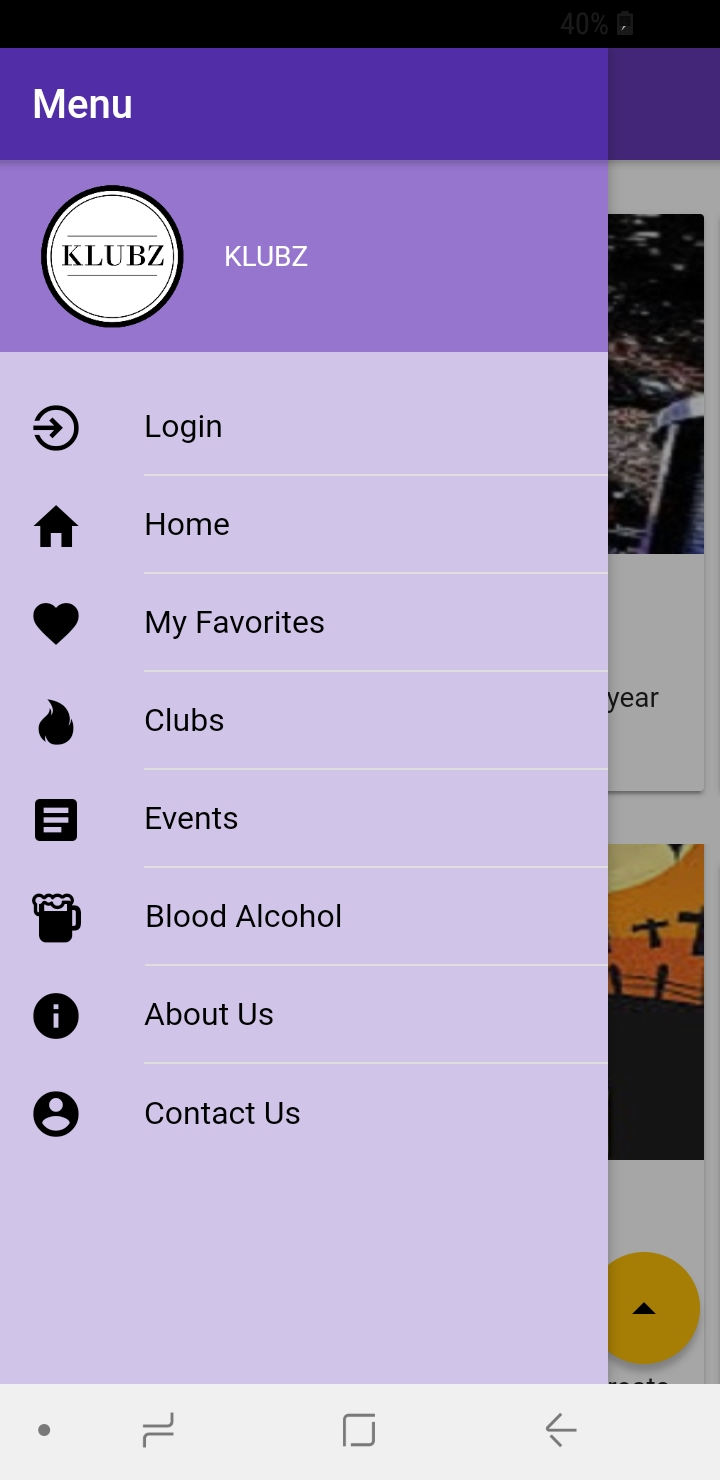
\includegraphics[width=\linewidth]{figures/Menu.jpg}
  \caption{Sidemenu}\label{fig:awesome_image6}
\endminipage
\end{figure}

\newpage
\section{UML}

Three different UML-Diagrams were created for this Pet Project:

\begin{figure}[H]
  \centering
    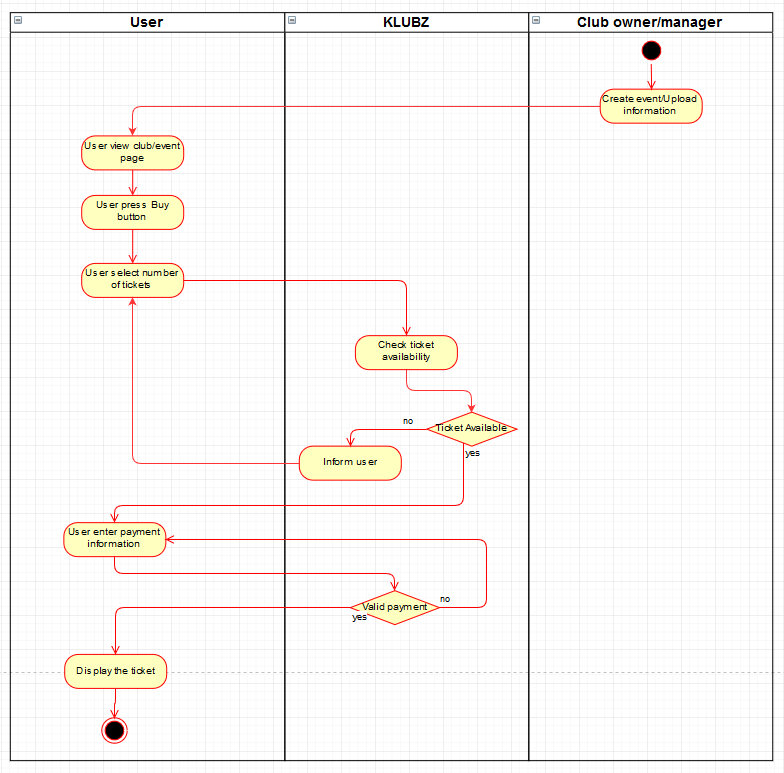
\includegraphics[width=1\textwidth]{figures/ActivityDiagram.png}
    \caption{Activity Diagram of the process Buying a Ticket}
\end{figure}

\begin{figure}[H]
  \centering
    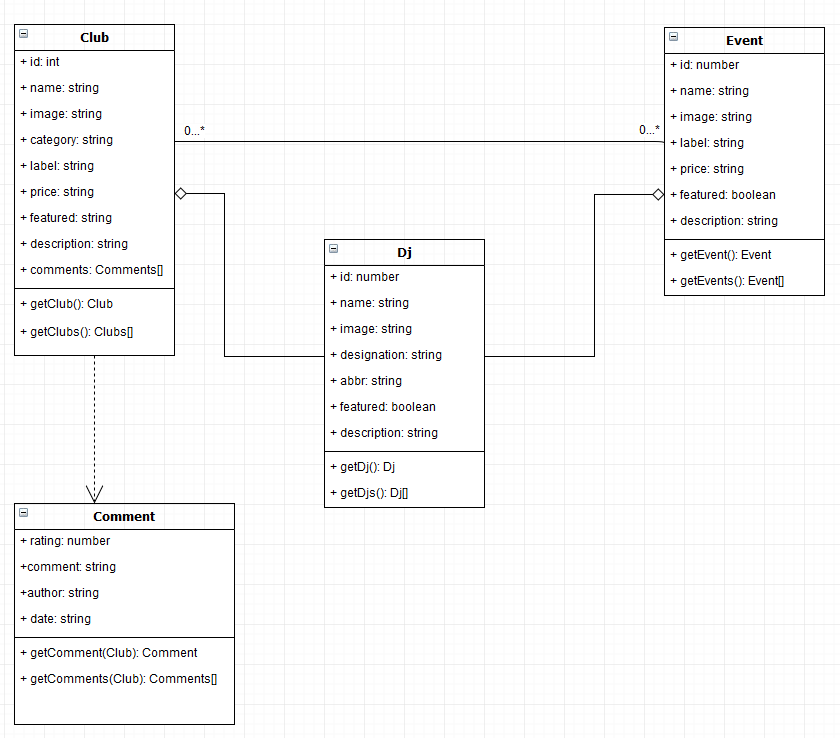
\includegraphics[width=1\textwidth]{figures/ClassDiagram.png}
    \caption{Class Diagram of Clubs, DJs, Events and Comments}
\end{figure}

\begin{figure}[H]
  \centering
    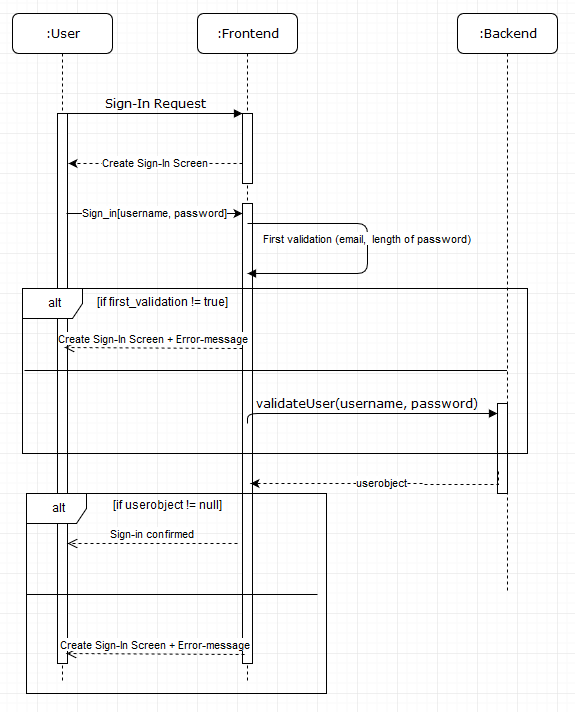
\includegraphics[width=1\textwidth]{figures/SequenceDiagram1.png}
    \caption{Sequence Diagram for Signing In }
\end{figure}

\begin{figure}[H]
  \centering
    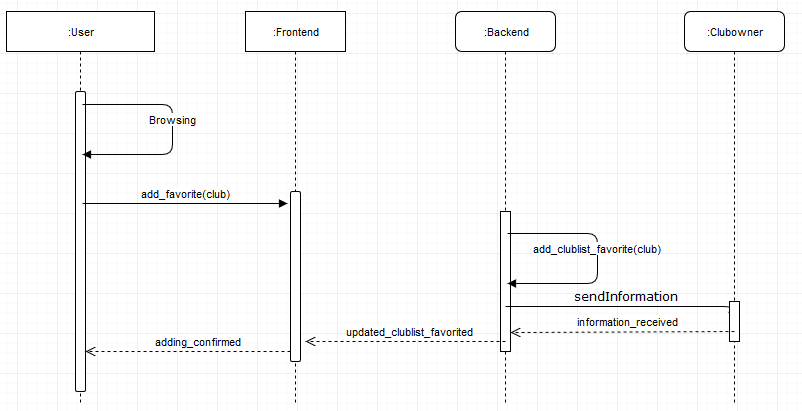
\includegraphics[width=1\textwidth]{figures/SequenceDiagram2.png}
    \caption{Sequence Diagram for Adding Favorites }
\end{figure}

\newpage
\section{Metrics}
The Metrics are obtained by running the Sonarcloud analysis for the project files. The results are shown in a screenshot of the Sonarcloud page \url{https://sonarcloud.io/dashboard?id=chrisschroer_pet_project} in the picture below.
\begin{figure}[H]
  \centering
    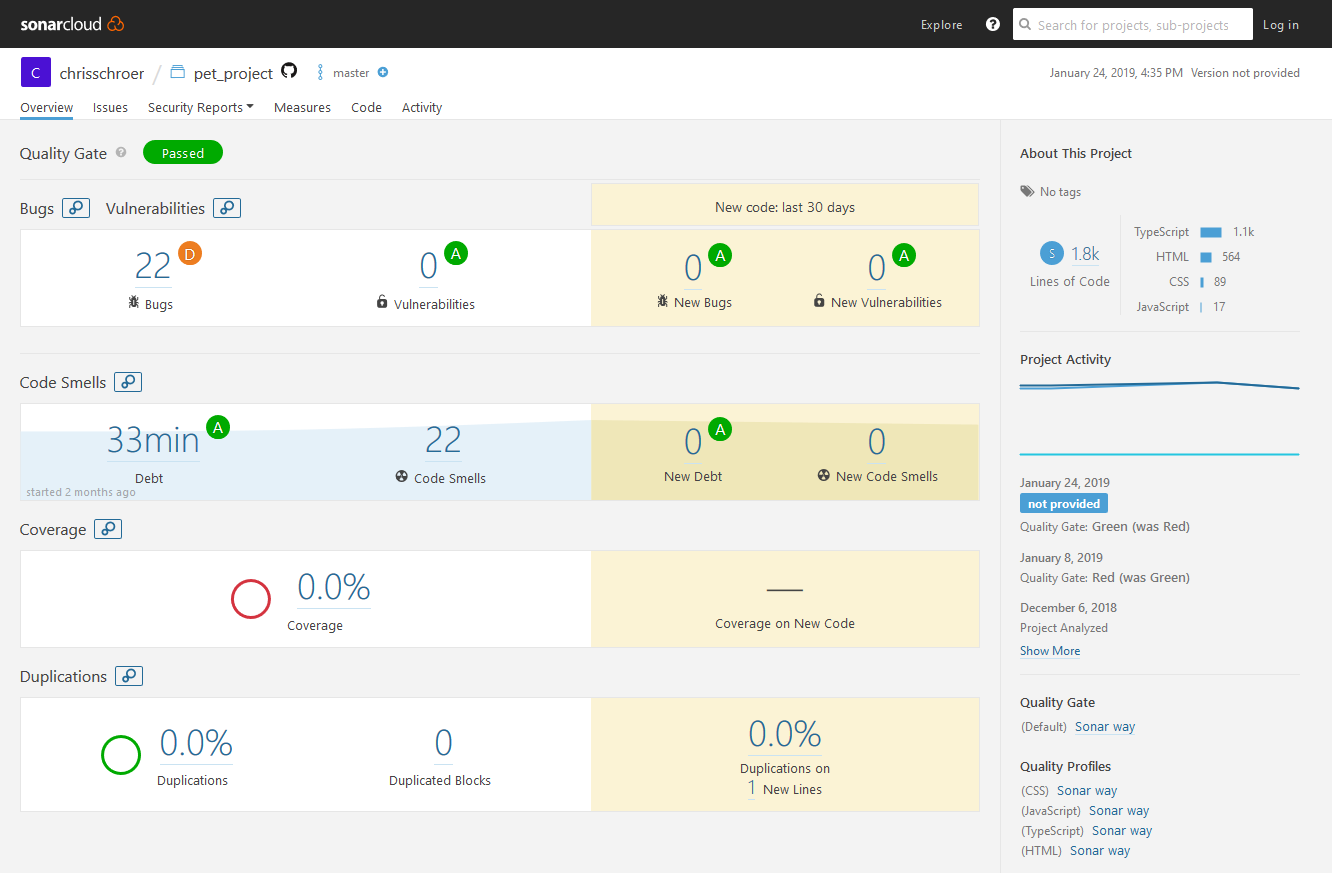
\includegraphics[width=1\textwidth]{figures/Sonarcloud.png}
    \caption{Screenshot of the metrics in Sonarcloud}
\end{figure}


The remaining bugs are usually of minor type and occur e.g. example because the Sonarcloud analysis expects an altitude parameter for every image. This parameter is not mandatory in the Ionic-Framework as picture sizes depend on the screen where the picture is shown.
\begin{figure}[H]
  \centering
    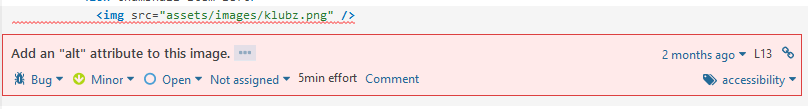
\includegraphics[width=1\textwidth]{figures/BugAlt.png}
    \caption{Minor Bug because of missing altitude parameter}
\end{figure}

A major bug occurs because Sonarcloud interprets the .scss-files wrong in which design definitions are set. These bugs can be ignored as these style defintions are important for several pages.
\begin{figure}[H]
  \centering
    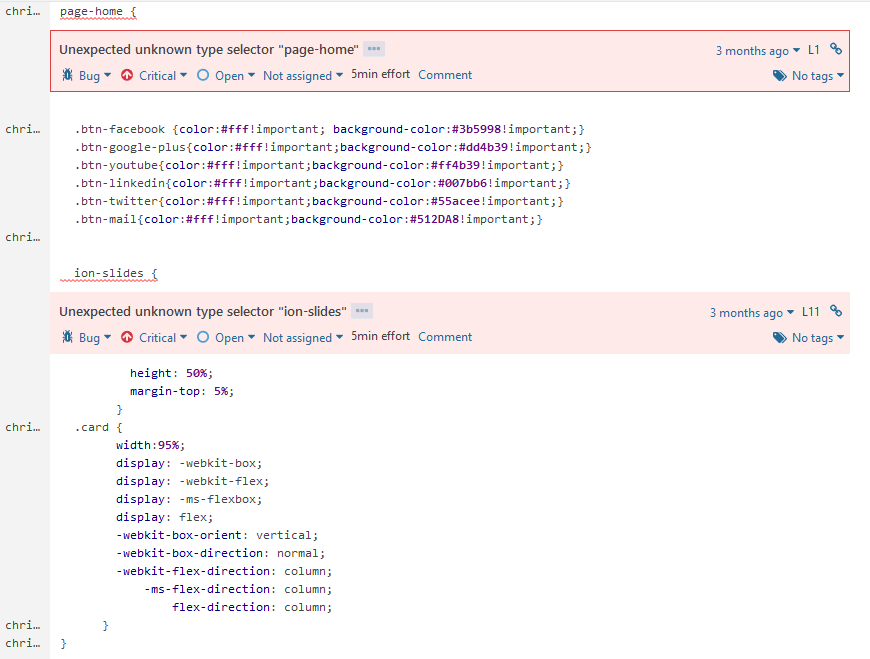
\includegraphics[width=1\textwidth]{figures/BugType.png}
    \caption{Major Bug because of unknown type selector}
\end{figure}

\newpage
\section{Clean Code Development}

Clean Code Development includes several principles for coding in an understandable and useful way to overcome issues in the further development of the code.

\subsection{Exception Handling}
Especially when working with servers and querying data, due to connection errors or wrong entries, different exceptions and errors can occur. Therefore, exception handling is important to enable an overall working product.
One example is given in the code snippet below. The function getClubs connects to baseurl/clubs and tries to retrieve all the data. If the query is successful, every club gets extracted for the presentation on the clubs-page. If no data is received, the error is catched and processed as an error message which is presented on the error page.
\begin{lstlisting}[language=javascript]
  getClubs(): Observable<Club[]> {
    return this.http.get(baseURL + 'clubs')
    .map(res => { return this.processHTTPMsgService.extractData(res); })
    .catch(error => { return this.processHTTPMsgService.handleError(error); });
  }
\end{lstlisting}

\subsection{Meaningful named variables}
Meaningful named variables are important to facilitate the understanding of the code. This reduces the debugging time and allows e.g. coworkers an easier overview of written code. In the following code snippet, the formgroup variables of the measurealc-page are named no\_beer, no\_wine and no\_cocktails, which stands for number of beer/wine/cocktails and allows an easy use for the further calculation of the alcohol level.

\begin{lstlisting}[language=javascript]
todo = {
    no_beer: 0,
    no_wine: 0,
    no_cocktails: 0,
    alc_level: 0
  }
\end{lstlisting}

\subsection{Open Closed Principle}

The Open-Close-Principle (OCP) states that a class should be open for new functions or adjustments while the existing functions mustn't be modified in order to keep their functionality. For the pet project, events have to be queried from the server. It could be one, all, or just the featured event, which are needed. These three cases could all be established in one function, but the prototype started with only retrieving one event. In the next step, the existing function had not been modified, but another one has been added (getClubs). In the further development, the third function (getFeaturedEvent()) has been added in order to not modify the functionality of the existing function. By defining these functions in the providers folder, they are accessible and only defined once. This demonstrates the OPC, as the functionality of the getEvent()-function had been proved only once, as the further function were added without modifying the first one.
\begin{lstlisting}[language=javascript]
getEvents(): Observable<Event[]> {
    return this.http.get(baseURL + 'events')
                    .map(res => { return this.processHTTPMsgService.extractData(res); })
                    .catch(error => { return this.processHTTPMsgService.handleError(error); });
  }

  getEvent(id: number): Observable<Event> {
    return  this.http.get(baseURL + 'events/'+ id)
                    .map(res => { return this.processHTTPMsgService.extractData(res); })
                    .catch(error => { return this.processHTTPMsgService.handleError(error); });
  }

  getFeaturedEvent(): Observable<Event> {
    return this.http.get(baseURL + 'events?featured=true')
                    .map(res => { return this.processHTTPMsgService.extractData(res)[0]; })
                    .catch(error => { return this.processHTTPMsgService.handleError(error); });
  }
\end{lstlisting}




\subsection{Interfaces - DRY}

In the pet project Interfaces are used for an easier access of frequently used instances. In this example, the Club interface is only assigned once and can be used anywhere else in the code just by importing the interface. It is an Don't-Repeat-Yourself (DRY) approach and prevents duplication of code.
\begin{lstlisting}[language=javascript]
import { Comment } from './comment';

export interface Club {
    id: number;
    name: string;
    image: string;
    category: string;
    label: string;
    price: string;
    featured: boolean;
    description: string;
    comments: Comment[];
}

\end{lstlisting}

\newpage
\subsection{Version Control - Git}

Version control is done with Git and Github for this pet project. It allows an simple and safe environment for the project code and could be easily edited or saved. With the commands git clone, the developers local folder is updated to the repository state. With git add, git commit and git push, the developer is able to update the repository.

\subsection{Continuous Delivery}
In \autoref{chap:cd} the use and the implementation of Continuous Delivery is described.


\subsection{Optimizations}

Another priciple states to be careful with optimizations. They should only be applied, if the optimization really result in a better product for the customer or are mandatory due to safety issues.\\
An example where these optimizations weren't necessary is explained in the following. 
The listings \autoref{lst:former} and \autoref{lst:latest} represent the two ways of initializing a formgroup. The first approach is the former one and the one I learned over one year ago in my Ionic course. The second one is the latest approach of initializing formgroups and I tried to implement in this way as well. This proved the Clean Code Principle, which states to be careful with optimizations. With the new structure of the newer approach of initialization, the reagarding functions had the be changed, too. This led to a waste of time to rewrite correctly performing functions and it made me realize that optimization are not always necessary. Here, the use of the newer approach did not result in a better UX and should have been avoided in terms of timesavings and code complexity.

\begin{lstlisting}[label = {lst:former}, language=javascript, caption={Former formgroup initialization},captionpos=b]
  this.commentForm = this.formBuilder.group({
    author: '',
    rating: 3,
    comment: ['', Validators.required],
  });
}

\end{lstlisting}


\begin{lstlisting}[label = {lst:latest},language=javascript, caption={Latest formgroup initialization},captionpos=b]
  todo = {
    no_beer: 0,
    no_wine: 0,
    no_cocktails: 0,
    alc_level: 0
  }
\end{lstlisting}



\newpage
\section{Build Management}

The Ionic Framework uses Cordova which includes Gradle to build and deploy apps. To build e.g. an Android App, the command\\
$ > \, ionic\, cordova\, add\, android $\\
needs to be run to add the Android platform the existing code. The command creates a platform/android directory, in which all necessary files for Android build are stored.\\
The final .apk-File for the App is created by running\\
$ > \, ionic\, cordova\, build\, android $\\
Afterwards, the App can be run by executing\\
$ > \, ionic\, cordova\, run\, android $ \\
if a suitable smartphone with an Android operating system in developer mode is connected to the PC via USB, the App is installed on the smartphone and started. If only an emulator of Android Studio is available, the App is started in the emulator.\\
For the whole Framework, there are several files that are involved in the build management.\\
In the main folder, the config.xml-File is stored. In addition to this general setting file, several build.gradle-Files are stored for each platform. The structure of the build.gradle-Files is shown in the picture below. In this pet project, the directory for the gradle-Files is /platforms/android...
\begin{figure}[H]
  \centering
    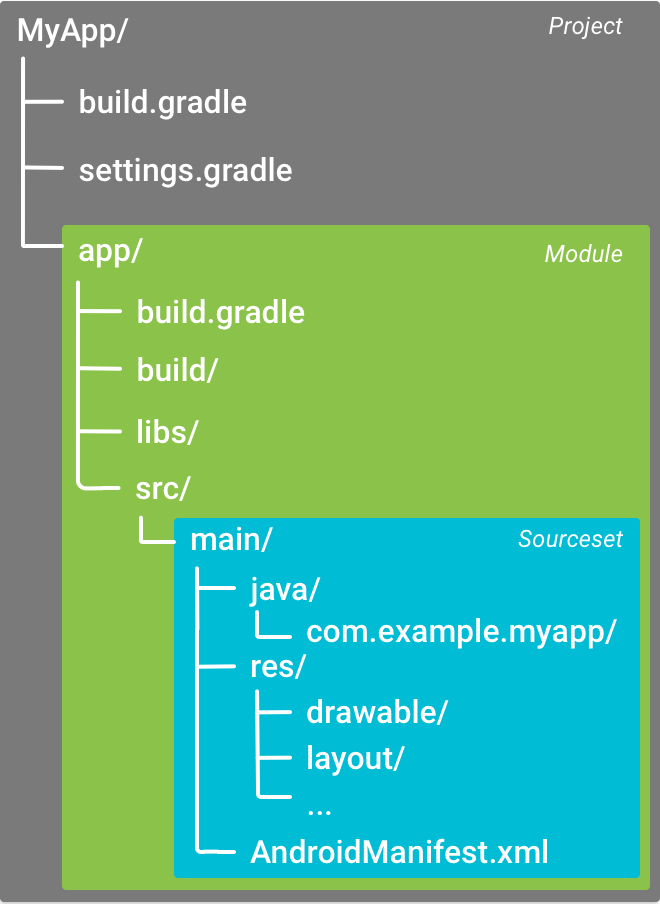
\includegraphics[width=0.5\textwidth]{figures/gradle_files.png}
    \caption{Structure of Build Management with Cordova}
\end{figure}
\subsection{config.xml-File}

The config.xml-File contains the settings which are identical for each of the platforms.
Included are the version, the name, the src-File and required plugins, e.g. Plugins for social sharing or the use of the camera.

\begin{lstlisting}[language=javascript]
<?xml version='1.0' encoding='utf-8'?>
<widget id="io.ionic.starter" version="0.0.3" xmlns="http://www.w3.org/ns/widgets" xmlns:cdv="http://cordova.apache.org/ns/1.0">
    <name>KLUBZ</name>
    <description>A nightlife app.</description>
    
.....

	<plugin name="cordova-plugin-email" spec="1.2.7" />
    <plugin name="cordova-plugin-x-socialsharing" spec="5.4.3">
        <variable name="ANDROID_SUPPORT_V4_VERSION" value="24.1.1+" />
    </plugin>
    <plugin name="cordova-plugin-camera" spec="4.0.3" />
</widget>
\end{lstlisting}


\subsection{Top-level build.gradle-File}

The top-level build.gradle file, located in the app project directory, defines build configurations that apply to all modules in the specific platform project. By default, the top-level build file uses the buildscript block to define the Gradle repositories and dependencies that are common to all modules in the project. The following code sample describes some settings and DSL elements you can find in the top-level build.gradle.\\
The allprojects category describes which SDK-Versions of Android are the minimum requirement (here Android 4.4) and which are actually targeted (always the latest one).

\begin{lstlisting}[language=javascript]
allprojects {
    repositories {
        maven {
            url "https://maven.google.com"
        }
        jcenter()
    }
    //This replaces project.properties w.r.t. build settings
    project.ext {
      defaultBuildToolsVersion="27.0.1" //String
      defaultMinSdkVersion=19 //Integer - Minimum requirement is Android 4.4
      defaultTargetSdkVersion=27 //Integer - We ALWAYS target the latest by default
      defaultCompileSdkVersion=27 //Integer - We ALWAYS compile with the latest by default
    }
}
\end{lstlisting}


\subsection{Module-level build.gradle-File}

The module-level build.gradle file, located in each project/module/ directory, allows you to configure build settings for the specific module it is located in. Configuring these build settings allows you to provide custom packaging options, such as additional build types and product flavors, and override settings in the main/ app manifest or top-level build.gradle file. In the following code snippet, the product flavors are defined for a free and a paid version of the app. These instructions are additional to the top-level File and gives the developer the opportunity to customize an app in several ways.

\begin{lstlisting}[language=javascript]
 /**
   * The productFlavors block is where you can configure multiple product flavors.
   * This allows you to create different versions of your app that can
   * override the defaultConfig block with their own settings. Product flavors
   * are optional, and the build system does not create them by default.
   *
   * This example creates a free and paid product flavor. Each product flavor
   * then specifies its own application ID, so that they can exist on the Google
   * Play Store, or an Android device, simultaneously.
   *
   * If you declare product flavors, you must also declare flavor dimensions
   * and assign each flavor to a flavor dimension.
   */

  flavorDimensions "tier"
  productFlavors {
    free {
      dimension "tier"
      applicationId 'com.example.myapp.free'
    }

    paid {
      dimension "tier"
      applicationId 'com.example.myapp.paid'
    }
  }

\end{lstlisting}
Description of some build.gradle-commands and how the structure is used.\\
Documentation of the build.gradle-Files in the Android structure\\
https://developer.android.com/studio/build/build-files\\

\subsection{Unit Tests}
Unit Tests in the Ionic Framework are not fully supported already and still in development, especially for using them with CLI-commands. That's why they are not implemented in this pet project as it would have been too time-consuming to get over all the issues while developing these tests.\\
A short example of a test within the Ionic Framework is given in the code snippet below. The main page is imported, afterwards newly created and in order to get to the default screen it is navigated to the main page. With the it-function, the test is conducted and it is checked if the title of the main page (Page One) is actually named 'Page One'.

\begin{lstlisting}[language=javascript]
import { Page } from './app.po';

describe('App', () => {
  let page: Page;

  beforeEach(() => {
    page = new Page();
  });

  describe('default screen', () => {
    beforeEach(() => {
      page.navigateTo('/');
    });

    it('should have a title saying Page One', () => {
      page.getPageOneTitleText().then(title => {
        expect(title).toEqual('Page One');
      });
    });
  })
});
\end{lstlisting}

\section{Continuous Delivery}\label{chap:cd}

The Jenkinsfile is located in the main folder in the repository on Github. In addition to environment preparing and building steps, there is also a Sonarcloud analysis step. If all steps are executed with success, a Slack notification to a private channel named $ \sharp$build is pushed. The steps of signing and publishing the APK-File do not contain valid pipeline code, but are important to be considered for building an App which should be published in an App Store.\\
The pipeline in Jenkins and the resulting Slack notification are shown in the below pictures:
\begin{figure}[H]
 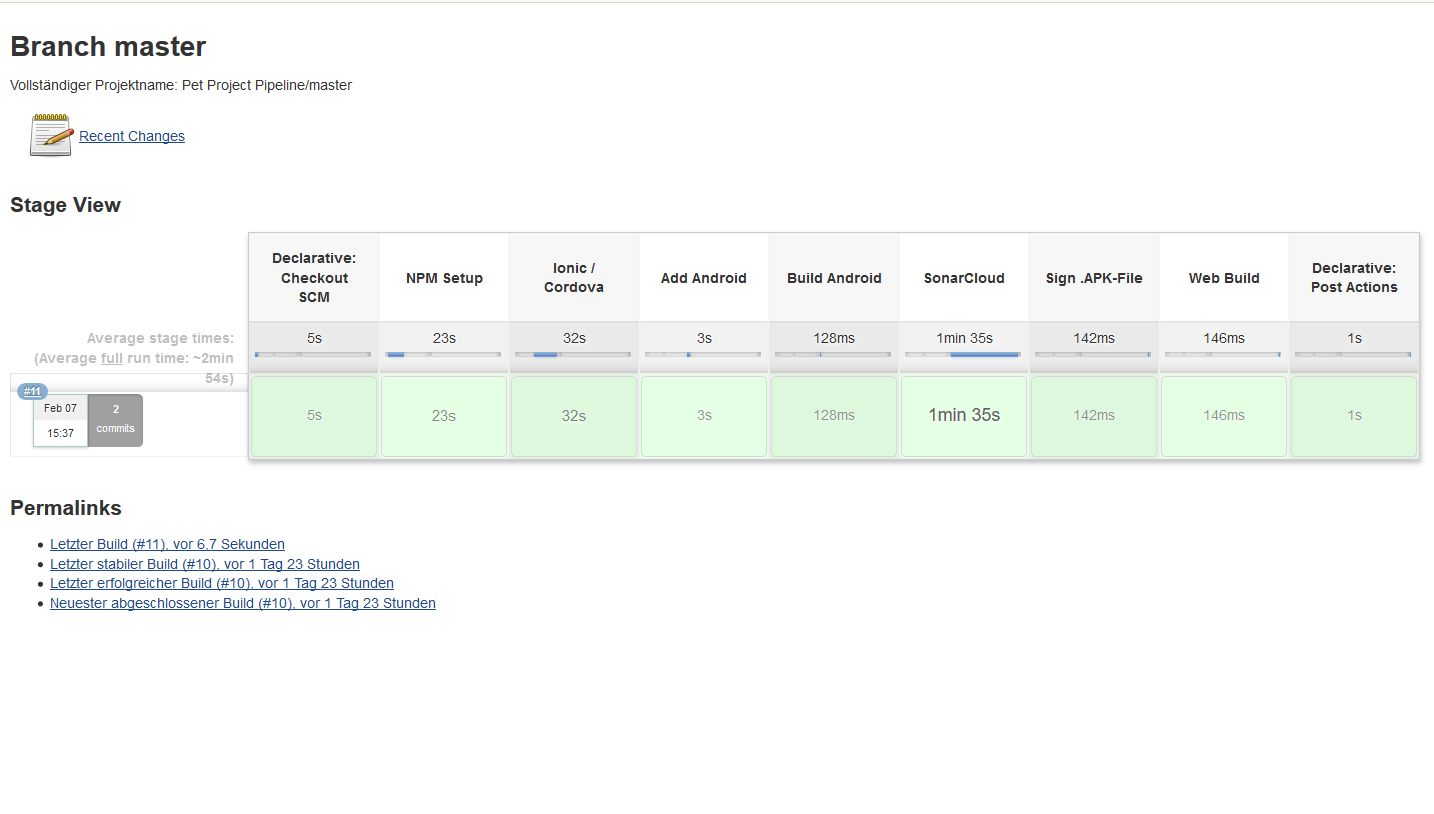
\includegraphics[width=\linewidth]{figures/Jenkins_Pipeline.PNG}
 \caption{Jenkins- Pipeline of a build success}\label{fig:awesome_image7}
\end{figure}
\begin{figure}[H]
 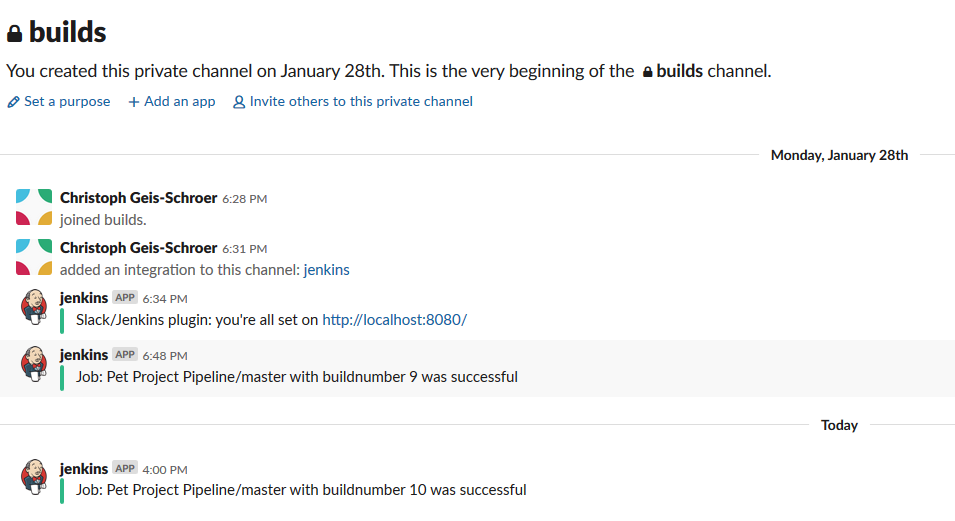
\includegraphics[width=\linewidth]{figures/Slack_Notification.PNG}
 \caption{Slack notification pushed by the Jenkinspipeline}\label{fig:awesome_image8}
\end{figure}

\section{DSL}
Domain Specific Languages are languages created to support a particular set of tasks, as they are performed in a specific domain.
Within this domain, DSLs can serve all sort of purposes and can be used in different contexts and by different kinds of users. Some DSLs are intended to be used by programmers, and therefore are more technical, while others are intended to be used by people with little programming expertise and therefore use less technical syntax.
\subsection{External}
External DSLs are used throughout the whole pet project within the .html or .css-files. An example is giving by the following two files.\\

HTML-File\\
\begin{lstlisting}
<ion-split-pane>
<ion-menu [content]="content">
  <ion-header>
    <ion-toolbar color="primary-dark">
      <ion-title>Menu</ion-title>
    </ion-toolbar>
  </ion-header>

  <ion-content class="background-pale">
    <ion-list>
      <ion-list-header color="primary-light" text-wrap>
          <ion-thumbnail item-left>
            <img src="assets/images/klubz.png" />
          </ion-thumbnail>
          <h3>KLUBZ</h3>
      </ion-list-header>
      <button color="primary-pale" menuClose ion-item (click)="openLogin()">
        <ion-icon name="log-in" item-left></ion-icon>
        Login
      </button>
      <button color="primary-pale" menuClose ion-item *ngFor="let p of pages" (click)="openPage(p)">
      <ion-icon [name]="p.icon" item-left></ion-icon>
        {{p.title}}
    </button>
    </ion-list>
  </ion-content>

</ion-menu>\\
\end{lstlisting}

CSS-File\\
The Cascading Style Sheet language defines the style which should be used to visualize a document. It can be used to define how an HTML document will appear on the screen like in the following example, where different background colors are defined.
\begin{lstlisting}
$lt-gray: #ddd;
$background-dark: #512DA8;
$background-light: #9575CD;
$background-pale: #D1C4E9;

.background-pale {
    background-color: $background-pale
}

.modal-open {
  pointer-events: auto !important;
}
\end{lstlisting}

\subsection{Internal}
Internal DSLs are seperated in Embedded DSLs and Generative DSLs. These internal DSLs are written inside an existing host language. Unlike an external DSL, the internal are limited by the syntax and programming model of the host language. Another possible usage of internal DSLs is to enhance the host language by using DSL techniques to solve a specific task in a facilitated way.


\section{Functional Programming}

The following paradigms of functional programs are explained / shown in the source code or by given examples.

\subsection{Final Data Structures}

Typescript does not support final data structures like they are known from Java. Therefore, other approaches have to be used to create immutable variables.\\
First: 	In a class with a private variable\\
\begin{lstlisting}[language=javascript]
export default class Person {
  readonly name: string
  readonly surname: string
  readonly city: string
    
  constructor (name: string, surname: string, city: string) {
    this.name = name
    this.surname = surname
    this.city = city
  }
}
\end{lstlisting}
Second:	A constant\\
exported interfaces?
\subsection{(mostly) Side Effect Free Functions}

All functions are side effect-free, e.g. the calculation function of the blood alcohol level always returns the same value for the same input. Non-side-effect free are the functions retrieving information from the NodeJS-Server. If the content changes on the server side, the return of the function will have another value than before the change.

\subsection{Higher Order Functions}

Examples
\begin{lstlisting}[language=javascript]
getClubs(): Observable<Club[]> {
    return this.http.get(baseURL + 'clubs')
    .map(res => { return this.processHTTPMsgService.extractData(res); })
    .catch(error => { return this.processHTTPMsgService.handleError(error); });
  }
\end{lstlisting}
.map() is a higher order function as it takes a function as an argument and applies it to all the responses which are returned when querying the Server. With this extractData(res)-function, the data gets extracted and is visible on the client side.

\subsection{Closures}

A closure is a persistent scope which holds on to local variables even after the code execution has moved out of that block. Languages which support closure (such as JavaScript, Swift, and Ruby) will allow you to keep a reference to a scope (including its parent scopes), even after the block in which those variables were declared has finished executing. To overcome this issue, a closure can be used by providing a reference to that block or function somewhere in the code.\\
The scope object and all its local variables are tied to the function and will persist as long as that function persists.
This gives us function portability. We can expect any variables that were in scope when the function was first defined to still be in scope when we later call the function, even if we call the function in a completely different context.\\
Closures provide much needed convenience, as otherwise we would be passing every single dependency of the function as an argument.

\begin{lstlisting}[language=javascript]
outer = function() {
  var a = 1;
  var inner = function() {
    console.log(a);
  }
  return inner; // this returns a function
}

var func_inner = outer(); // execute outer to get inner 
func_inner();
\end{lstlisting}

In the example code snippet a function within a function is declared. The inner function gains access to all the outer function's local variables, including a. The variable a is in scope for the inner function.\\
Without a closure, when a function exits, all its local variables are garbage collected and not persistent anymore. But, if the inner function is returned and assigned to a variable func\_inner so that it persists after outer has exited, all of the variables that were in scope when inner was defined also persist. The variable a has been closed over and is therefore within a closure.\\
One special note: The variable a is totally private to func\_inner. This is a way of creating private variables in a functional programming language such as JavaScript.\\
By running this sample, the variable will be printed which results in a printed ''1''.

\subsection{Anonymous functions}

An anonymous function is a function that was declared without any named identifier to refer to it. As such, an anonymous function is usually not accessible after its initial creation.
 
\begin{lstlisting}[language=javascript]
// Named function
function add(x, y) {
    return x + y;
}

// Call named function
console.log(add(5,10));

// Anonymous function
let myAdd = function(x, y) { return x + y; };

// You can call it like this
console.log(myAdd(5,10));
\end{lstlisting}

% --------------------------------------------------------------
%     You don't have to mess with anything below this line.
% --------------------------------------------------------------
 
\end{document}